\documentclass{beamer}
\usepackage[utf8]{inputenc}
\usepackage{listings}
\usepackage{relsize}
\usepackage{graphicx}

\usetheme{Montpellier}

\newcommand{\code}[1]{\texttt{#1}}

\lstset{
 basicstyle=\tiny,
 showspaces=false,
 showstringspaces=false,
 frame=single,
 stringstyle=\ttfamily
}

\title{Spring Batch Workshop}
\author{Arnaud Cogoluègnes}
\institute{Consultant with Zenika, Co-author Spring Batch in Action}

\begin{document}

\begin{frame}
\titlepage
\end{frame}

\section{Overview}

\begin{frame}
\frametitle{Overview}
\begin{itemize}
	\item This workshop highlights Spring Batch features
	\item Problem/solution approach
	\begin{itemize}
		\item A few slides to cover the feature
		\item A project to start from, just follow the TODOs
	\end{itemize}
	\item Prerequisites
	\begin{itemize}
		\item Basics about Java and Java EE
		\item Spring: dependency injection, enterprise support
	\end{itemize}
	\item https://github.com/acogoluegnes/Spring-Batch-Workshop
\end{itemize}

\end{frame}

\begin{frame}
\frametitle{License}

This work is licensed under the Creative Commons Attribution-NonCommercial-ShareAlike 3.0 
Unported License. 

To view a copy of this license, 
visit http://creativecommons.org/licenses/by-nc-sa/3.0/ or 
send a letter to Creative Commons, 444 Castro Street, Suite 900, Mountain View, 
California, 94041, USA.

\end{frame}

\section{IDE set up}

\begin{frame}
\frametitle{Follow the TODOs}
\begin{itemize}
 \item Track the TODO in the *-start projects!
 \item It's easier with support from the IDE
\end{itemize}

\begin{figure}
\begin{center}
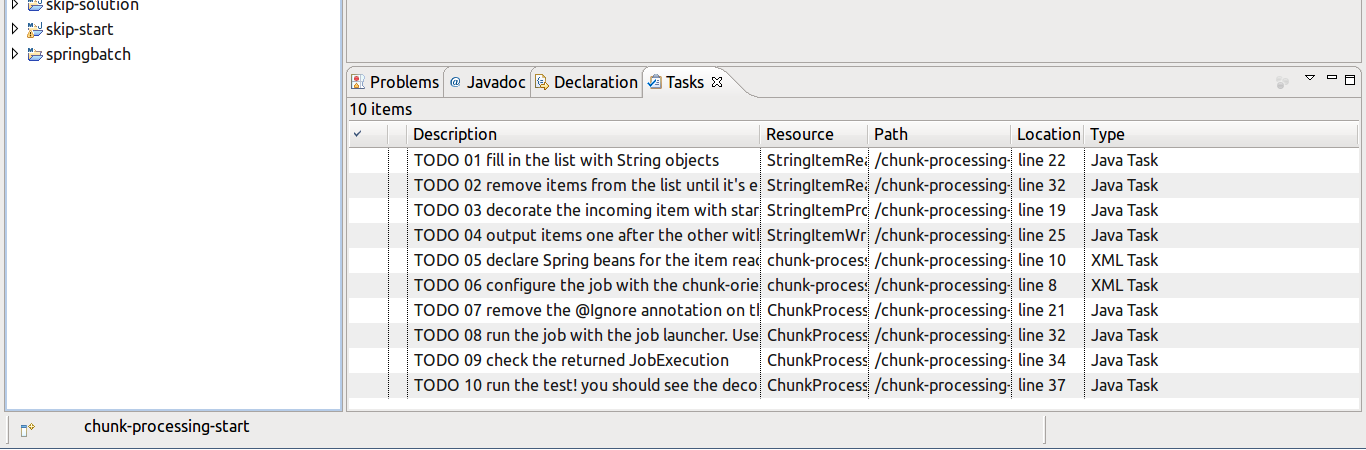
\includegraphics[width=10cm]{figures/tasks.png}
\end{center}
\end{figure}
 
\end{frame}

\begin{frame}
\frametitle{TODO with Eclipse}
\begin{itemize}
 \item Window \textgreater \space Preferences \textgreater \space ``tasks tag'' in filter   
\end{itemize}

\begin{figure}
\begin{center}
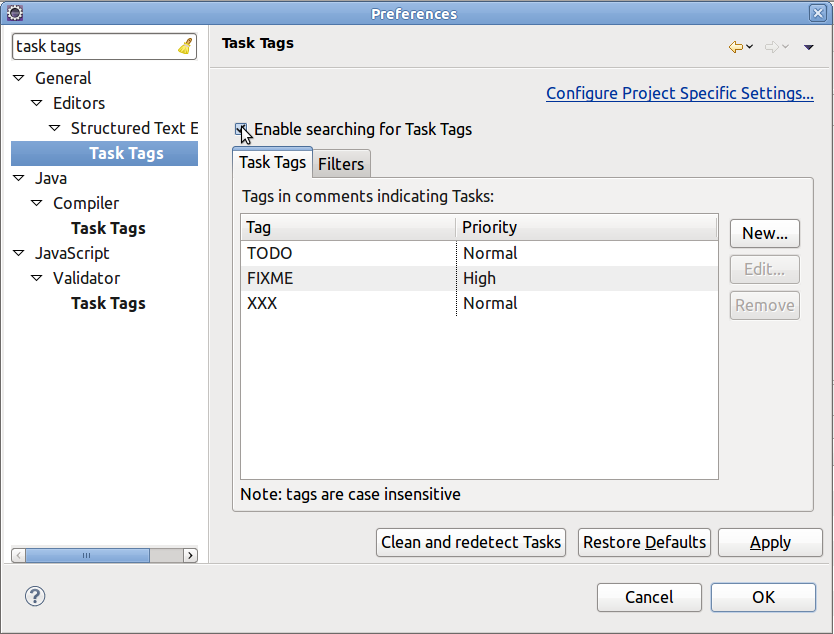
\includegraphics[width=8cm]{figures/enable-task-tags.png}
\end{center}
\end{figure}

\end{frame}
 
\begin{frame}
\frametitle{TODO with Eclipse}
\begin{itemize}
 \item Open the ``Tasks'' view 
 \item click on the down arrow on the right
 \item ``configure contents''
\end{itemize}

\begin{figure}
\begin{center}
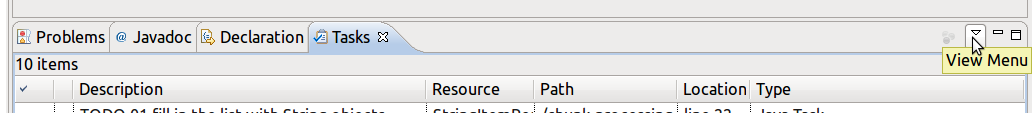
\includegraphics[width=8cm]{figures/configure-content.png}
\end{center}
\end{figure}

\end{frame}

\begin{frame}
\frametitle{TODO with Eclipse}
\begin{itemize}
 \item Check ``TODOs'' on the left
 \item Check ``On any element in the same project'' on the right (scope)
\end{itemize}

\begin{figure}
\begin{center}
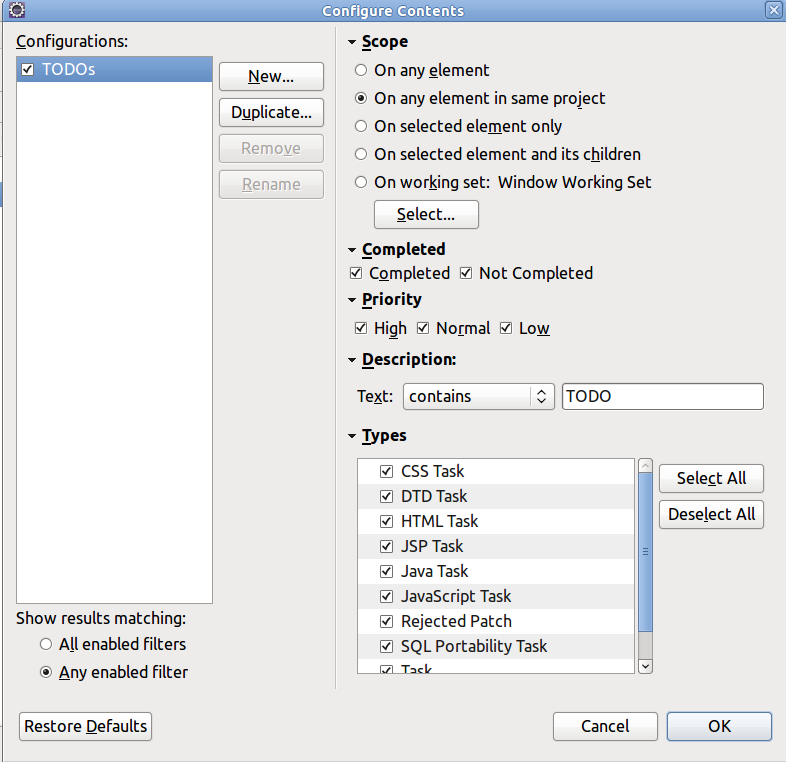
\includegraphics[width=5cm]{figures/content.png}
\end{center}
\end{figure}


\end{frame}
\section{Spring support in IDE}

\begin{frame}
\frametitle{Spring support in IDE is a +}

\begin{itemize}
 \item e.g. code completion in SpringSource Tool Suite
\end{itemize}

\begin{figure}
\begin{center}
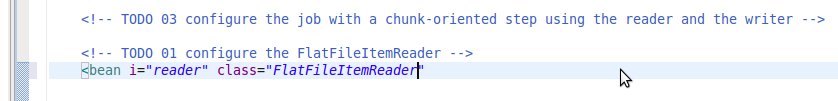
\includegraphics[width=10cm]{figures/before-cc.png}
\end{center}
\end{figure}

\begin{center}
\begin{picture}(0,0)
\put(0,15){\vector(0,-1){15}} 
\end{picture}
\end{center}

\begin{figure}
\begin{center}
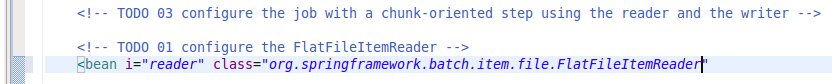
\includegraphics[width=10cm]{figures/after-cc.png}
\title{Code completion in SpringSource Tool Suite}
\end{center}
\end{figure}
 
\end{frame}
\section{Spring Batch overview}

\begin{frame}
\frametitle{Basic features for batch applications}
\begin{itemize}
	\item Read – process – write large amounts of data, efficiently
	\item Ready-to-use components to read from/write to
	\begin{itemize}
		\item Flat/XML files
		\item Databases (JDBC, Hibernate, JPA, iBatis)
		\item JMS queues
		\item Emails
	\end{itemize}
	\item Numerous extension points/hooks	
\end{itemize}

\end{frame}

\begin{frame}
 \frametitle{Advanced features for batch applications}
 \begin{itemize}
  \item Configuration to skip/retry items
  \item Execution metadata
   \begin{itemize}
     \item Monitoring
     \item Restart after failure
   \end{itemize}
  \item Scaling strategies
   \begin{itemize}
     \item Local/remote
     \item Partitioning, remote processing
   \end{itemize}
\end{itemize}
\end{frame}


\section{Hello World}

\begin{frame}
 \begin{itemize}
  \item Problem: getting started with Spring Batch
  \item Solution: writing a simple ``Hello World'' job
 \end{itemize}
\end{frame}

\begin{frame}
 \frametitle{Structure of a job}
 \begin{itemize}
  \item A Spring Batch job is made of steps
  \item The Hello World job has one step
  \item The processing is implemented in a \code{Tasklet}
 \end{itemize}
\end{frame}

\begin{frame}[fragile]
\frametitle{The Hello World \code{Tasklet}}
\begin{javacode}
public class HelloWorldTasklet implements Tasklet {

  @Override
  public RepeatStatus execute(
      StepContribution contribution,
      ChunkContext chunkContext) throws Exception {
    System.out.println("Hello world!");
    return RepeatStatus.FINISHED;
  }

}
\end{javacode}
\end{frame}

\begin{frame}[fragile]
\frametitle{The configuration of the Hello World job}
\begin{xmlcode}
<batch:job id="helloWorldJob">
  <batch:step id="helloWorldStep">
    <batch:tasklet>
      <bean class="c.z.workshop.springbatch.HelloWorldTasklet" />
    </batch:tasklet>
  </batch:step>
</batch:job>
\end{xmlcode}

\begin{itemize}
 \item Notice the \code{batch} namespace
\end{itemize}

\end{frame}

\begin{frame}[fragile]
\frametitle{Spring Batch needs some infrastructure beans}
\begin{itemize}
 \item Let's use the typical test configuration
\end{itemize}

\begin{xmlcode}
<bean id="transactionManager"
      class="o.s.b.support.transaction.ResourcelessTransactionManager"
      />

<bean id="jobRepository"   
      class="o.s.b.core.repository.support.MapJobRepositoryFactoryBean" 
      />

<bean id="jobLauncher"
      class="o.s.b.core.launch.support.SimpleJobLauncher">
  <property name="jobRepository" ref="jobRepository" />
</bean>
\end{xmlcode}
\end{frame}

\begin{frame}[fragile]
\frametitle{Running the test in a JUnit test}

\begin{javacode}
@RunWith(SpringJUnit4ClassRunner.class)
@ContextConfiguration("/hello-world-job.xml")
public class HelloWorldJobTest {

  @Autowired
  private Job job;

  @Autowired
  private JobLauncher jobLauncher;

  @Test public void helloWorld() throws Exception {
    JobExecution execution = jobLauncher.run(job, new JobParameters());
    assertEquals(ExitStatus.COMPLETED, execution.getExitStatus());
  }
}
\end{javacode}
\end{frame}

\section{Chunk processing}

\begin{frame}
 \begin{itemize}
  \item Problem: processing large amounts of data efficiently
  \item Solution: using chunk processing
 \end{itemize}
\end{frame}

\begin{frame}
 \frametitle{What is chunk processing?}
 \begin{itemize}
  \item Batch jobs often read, process, and write items
  \item e.g.
  \begin{itemize}
    \item Reading items from a file
    \item Then processing (converting) items
    \item Writing items to a database  
  \end{itemize}
  \item Spring Batch calls this ``chunk processing''
  \item a chunk = a set of items
 \end{itemize}
\end{frame}


\begin{frame}
 \frametitle{Chunk processing with Spring Batch}
 \begin{itemize}
  \item Spring Batch
  \begin{itemize}
    \item handles the iteration logic
    \item uses a transaction for each chunk
    \item lets you choose the chunk size
    \item defines interfaces for each part of the processing
  \end{itemize}
 \end{itemize}
\end{frame}


\begin{frame}[fragile]
\frametitle{The reading phase}
\begin{itemize}
 \item Spring Batch creates chunks of items by calling \code{read()}
 \item Reading ends when \code{read()} returns \code{null}
\end{itemize}

\lstset{language=Java}
\begin{lstlisting}
public interface ItemReader<T> {

  T read() throws Exception, UnexpectedInputException, 
                  ParseException, NonTransientResourceException;

}
\end{lstlisting}
\end{frame}

\begin{frame}[fragile]
\frametitle{The processing phase}
\begin{itemize}
 \item Once a chunk is created, items are sent to the processor
 \item Optional
\end{itemize}

\lstset{language=Java}
\begin{lstlisting}
public interface ItemProcessor<I, O> {

  O process(I item) throws Exception;

}
\end{lstlisting}
\end{frame}

\begin{frame}[fragile]
\frametitle{The writing phase}
\begin{itemize}
 \item Receives all the items of the chunk
 \item Allows for batch update (more efficient)
\end{itemize}

\lstset{language=Java}
\begin{lstlisting}
public interface ItemWriter<T> {

  void write(List<? extends T> items) throws Exception;

}
\end{lstlisting}
\end{frame}

\begin{frame}
 \frametitle{An example}
 \begin{itemize}
  \item Let's implement a (too?) simple chunk-oriented step!  
 \end{itemize}
\end{frame}

\begin{frame}[fragile]
\frametitle{The \code{ItemReader}}
\lstset{language=Java}
\begin{lstlisting}
public class StringItemReader implements ItemReader<String> {

  private List<String> list;

  public StringItemReader() {
    this.list = new ArrayList<String>(Arrays.asList(
      "1","2","3","4","5","6","7")
    );
  }

  @Override
  public String read() throws Exception, UnexpectedInputException,
                         ParseException, NonTransientResourceException {
    return !list.isEmpty() ? list.remove(0) : null;
  }
}
\end{lstlisting}
\end{frame}

\begin{frame}[fragile]
\frametitle{The \code{ItemProcessor}}
\lstset{language=Java}
\begin{lstlisting}
public class StringItemProcessor implements ItemProcessor<String, String> {

  @Override
  public String process(String item) throws Exception {
    return "*** "+item+" ***";
  }

}
\end{lstlisting}
\end{frame}

\begin{frame}[fragile]
\frametitle{The \code{ItemWriter}}
\lstset{language=Java}
\begin{lstlisting}
public class StringItemWriter implements ItemWriter<String> {

  private static final Logger LOGGER =
    LoggerFactory.getLogger(StringItemWriter.class);

  @Override
  public void write(List<? extends String> items) throws Exception {
    for(String item : items) {
      LOGGER.info("writing "+item);
    }
  }

}
\end{lstlisting}
\end{frame}

\begin{frame}[fragile]
\frametitle{Configuring the job}
\lstset{language=XML}
\begin{lstlisting}
<batch:job id="chunkProcessingJob">
  <batch:step id="chunkProcessingStep">
    <batch:tasklet>
      <batch:chunk reader="reader" processor="processor" writer="writer"
                   commit-interval="3"
      />
    </batch:tasklet>
  </batch:step>
</batch:job>

<bean id="reader" class="com.zenika.workshop.springbatch.StringItemReader" />

<bean id="processor" 
      class="com.zenika.workshop.springbatch.StringItemProcessor" />

<bean id="writer" class="com.zenika.workshop.springbatch.StringItemWriter" />
\end{lstlisting}
\end{frame}

\begin{frame}
 \frametitle{Considerations}
 \begin{itemize}
  \item Do I always need to write my \code{ItemReader}/\code{Processor}/\code{Writer}?
  \item No, Spring Batch provides ready-to-use components for common datastores
  \begin{itemize}
    \item Flat/XML files, databases, JMS, etc.
  \end{itemize}
  \item As an application developer, you
  \begin{itemize}
    \item Configure these components
    \item Provides some logic (e.g. mapping a line with a domain object)
  \end{itemize}
 \end{itemize}
\end{frame}

\begin{frame}
 \frametitle{Going further...}
 \begin{itemize}
  \item Reader/writer implementation for flat/XML files, database, JMS
  \item Skipping items when something goes wrong
  \item Listeners to react to the chunk processing  
 \end{itemize}
\end{frame}



\end{document}

